\documentclass[a4paper,11pt,fleqn]{report}

\usepackage{acronym}
\usepackage{amsmath,amssymb,amsfonts}
\usepackage{booktabs}
\usepackage[dvipsnames]{xcolor}
\usepackage[margin=28mm]{geometry}
\usepackage{graphicx}
%	\graphicspath{
%		{.../Graphics/}
%	}
\graphicspath{{graphics/}}
\usepackage{hyperref}
	\hypersetup{
		colorlinks=true,
		linkcolor=blue,
		filecolor=blue,
		urlcolor=blue,
		citecolor=blue
	}
\usepackage[sort&compress]{natbib}
	\bibliographystyle{apalike}
%\usepackage[mark]{gitinfo2}
%\renewcommand{\gitMark}{Branch:\,\gitBranch\,@\,\gitAbbrevHash{}; Author:\,\gitAuthorName; Date:\,\gitAuthorIsoDate~\textbullet{}}
\usepackage{url}

\begin{document}
%===============================================================
% Frontmatter and title page to be added manually at the end
%===============================================================
\thispagestyle{empty}
\begin{center}
{\huge \textit{`e-casa'} - Eco-friendly Household Waste System\\Part II}
\vspace{20mm} \\
{\Large Group 6}
\vfill

A project report in partial fulfilment of the requirements for the subject\\
\vspace{10mm}
{\Large \textsc{Systems Engineering (BSS 410)}} \\
\vfill
%
in the \\
\vspace{20mm}
%
{\Large \textsc{Faculty of Engineering, Built Environment, and \\ 
Information Technology}}\\
%
\vspace{10mm}
{\Large\textsc{University of Pretoria}} \\
%
\vfill
%
\today
\end{center}

\textit{`e-casa'} - Eco-friendly Household Waste System
\pagenumbering{roman}

\chapter*{Executive Summary}
The aim of this project is to create a household waste system System of that will not only reduce the waste produced by a generic household but do so by increasing value to the user. The final deliverable for this project will be a report that details the needs analysis, conceptual design, feasibility and risk assessment of the designed system. The coneptual design will be done with the use of \textit{Core 9} to capture all identified needs accurately and produce system design documentation.

\tableofcontents
\listoffigures\addcontentsline{toc}{chapter}{List of Figures}
\listoftables\addcontentsline{toc}{chapter}{List of Tables}

\chapter*{Acronyms}
\addcontentsline{toc}{chapter}{Acronyms}
\begin{acronym}[ABCDEF]
\acro{e-casa}{Eco-friendly Household Waste System}
\acro{FBD}{Functional Block Diagram}
\acro{SD}{System Dynamics}
\end{acronym}

\chapter{Introduction and Background}
\pagenumbering{arabic}
\setcounter{page}{1}
\acresetall

\section{Problem Background} \label{sec: Problem Background}
Households consume a variety of products and create different wastes. Products may take the form of food items, municipal water, electricity and other consumables which are either used up or discarded after use. Products discarded after use, such as excess food, food and beverage packaging and water exit the household as forms of waste.  Food clippings from preparing dinner or paper-based packaging is often discarded into dustbins alongside plastic and other waste types to be collected and transported to a dump site. Water used at bathroom sinks or showers is sent directly to the the municipal water system after use to be disposed of. Each type of waste generated by a typical residential household requires proceeding systems that will either store, repurpose or discard the waste.
  
Recent trends have made the consumer market ecologically aware of their own waste generation and many systems have been created to reduce the total waste output of a household. Such products include grey water systems, recycling bins and compost containers. There is a growing need for these means to be adpoted but presently no solution on the market that integrates all means into one comprehensive system for homeowners.
  
Because these systems operate independently, the outputs of one system are often not used as inputs to another. Integrating these systems to operate together could provide more value to the user and further reduce household waste. For example: using food clippings (to create a compost heap) and grey water to grow vegetables in one's garden instead of disposing food clippings in a general waste bin and discarding water to the municipal water system directly after its first use. This eliminates the need for compost to be purchased from a store and reduces water consumption.

\section{Project Objective} \label{sec: Project Objective}
The objective of this project is therefore to investigate the possibility of integrating these different systems as one. The intention is to determine whether the potential cost and resource use savings to be earned from such an integrated system outweigh the financial cost and initial inconvenience to install.

\chapter{Concept Development Stage}
\section{Needs Analysis Phase} \label{sec: Needs Analysis Phase}
\subsection{Operational Need Analysis} \label{Ssec: Operational Need}
\ac{e-casa} is a sustainable household waste management system intended to fulfuill the increasingly prevalent need for sustainable living. The need for individuals and households to consume and dispose of resources in a more sustainable manner is becoming ever more pertinent because of increasing strain on the world's most essential natural resources such as water and fossil fuels. The need is driven by the requirement for individuals (and society as a whole) to reduce their negative impact on the environment by re-use, recycling and minimising resource use as these natural resources become more scarce. Successfully meeting this need will not only improve living conditions for societies but importantly alleviate pressure on governments and municipalities who have to manage and distribute these water and electricity resources to the public.
Although regulation does not yet fully drive this need, government encourages and sometimes imposes restrictions to encourage responsible water and electricity use. This is important to develop a sustainable mindset and awareness of waste generation. Because regulation is still limited on the use of these resources, the onus lies with society and individuals who are aware of and want to mitigate their negative impact on the environment.

\ac{e-casa} is aimed at fulfilling the operational need of sustainable living for households by providing a system that makes it possible to manage and dispose of waste responsibly while simultaneously minimising water consumption. \ac{e-casa} is also expected to provide long-term financial benefits to the user in the form of reduced water consumption costs and grocery bills (with some homegrown foods). Furthermore, there is the expected intangible benefit of the system - knowing one's adverse impact on the environment is mitigated.

Due to a lack of solutions currently on the market, there is an opportunity to enter a gap in the market with \ac{e-casa}. However, this gap is anticipated to be small in size as this product will mainly be aimed at high income individuals aware of (and wanting to reduce) their impact on the environment. There is also an opportunity to market this system as a product to middle class individuals who have sufficient capital to purchase such a system now in order to reap the aforementioned financial savings down the line. However, this extension will likely only be possible if the initial cost of the system is not too high for these individuals and the financial savings are substantial enough to persuade this group.\\


\subsection{Operational Objectives}
The overarching objective that \ac{e-casa} is intended to fulfil is to provide sustainable household waste management. This objective is deconstructed into three primary objectives, namely: \textit{Provide Waste Sortation and Storage}, \textit{Reduce Water Consumption} and \textit{Provide long-term cost savings}. Figure~\ref{fig: ecasaOT} shows the operational objectives of the \ac{e-casa} system.\\

\textcolor{red}{*We need an objective tree of our own here that resembles Figure~\ref{fig: ObjectiveTreeStructure}. Figure~\ref{fig: ecasaOT} is a work in progress of that so far.}

\begin{figure}[h!]
\begin{center}
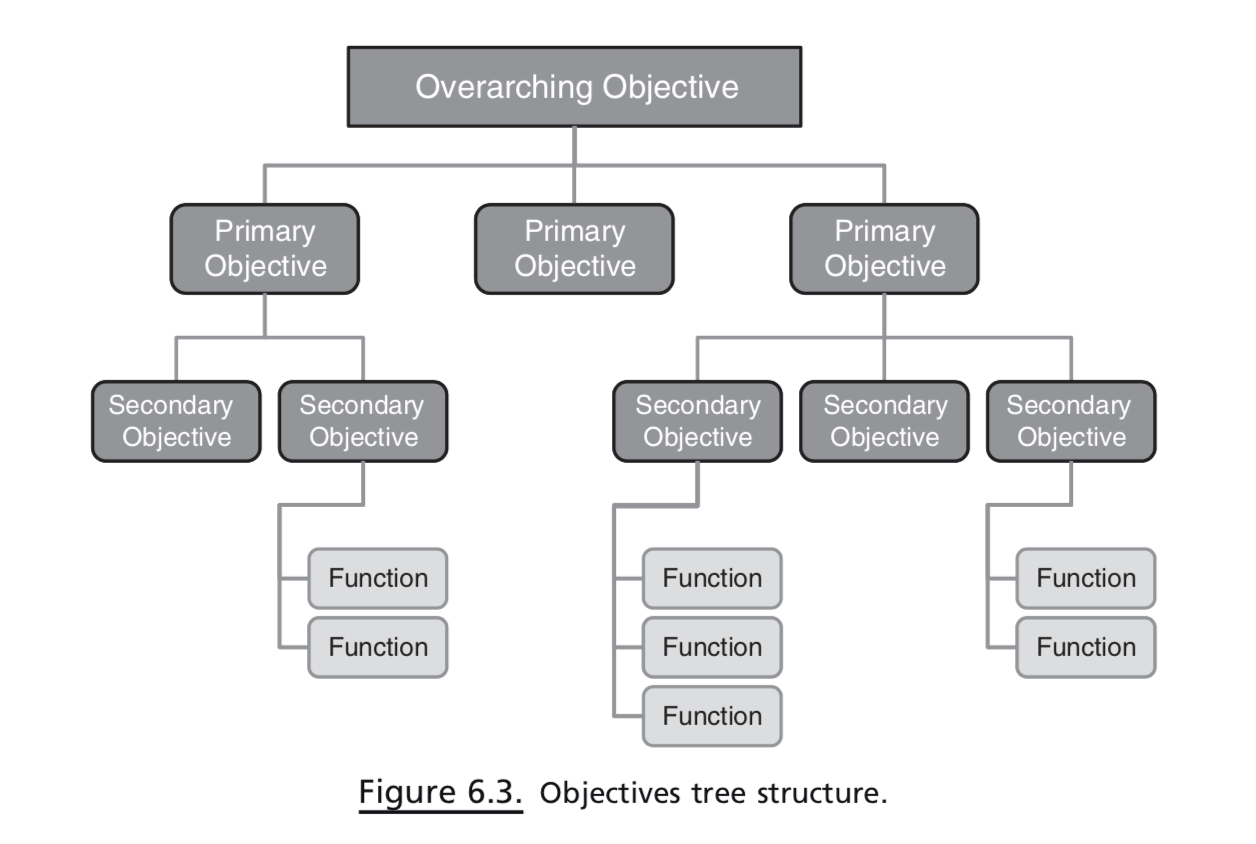
\includegraphics[scale = 0.6]{Objective_Tree_Structure.png}
\caption{Objective Tree Structure}
\label{fig: ObjectiveTreeStructure}
\end{center}
\end{figure}

\begin{figure}[h!]
\begin{center}
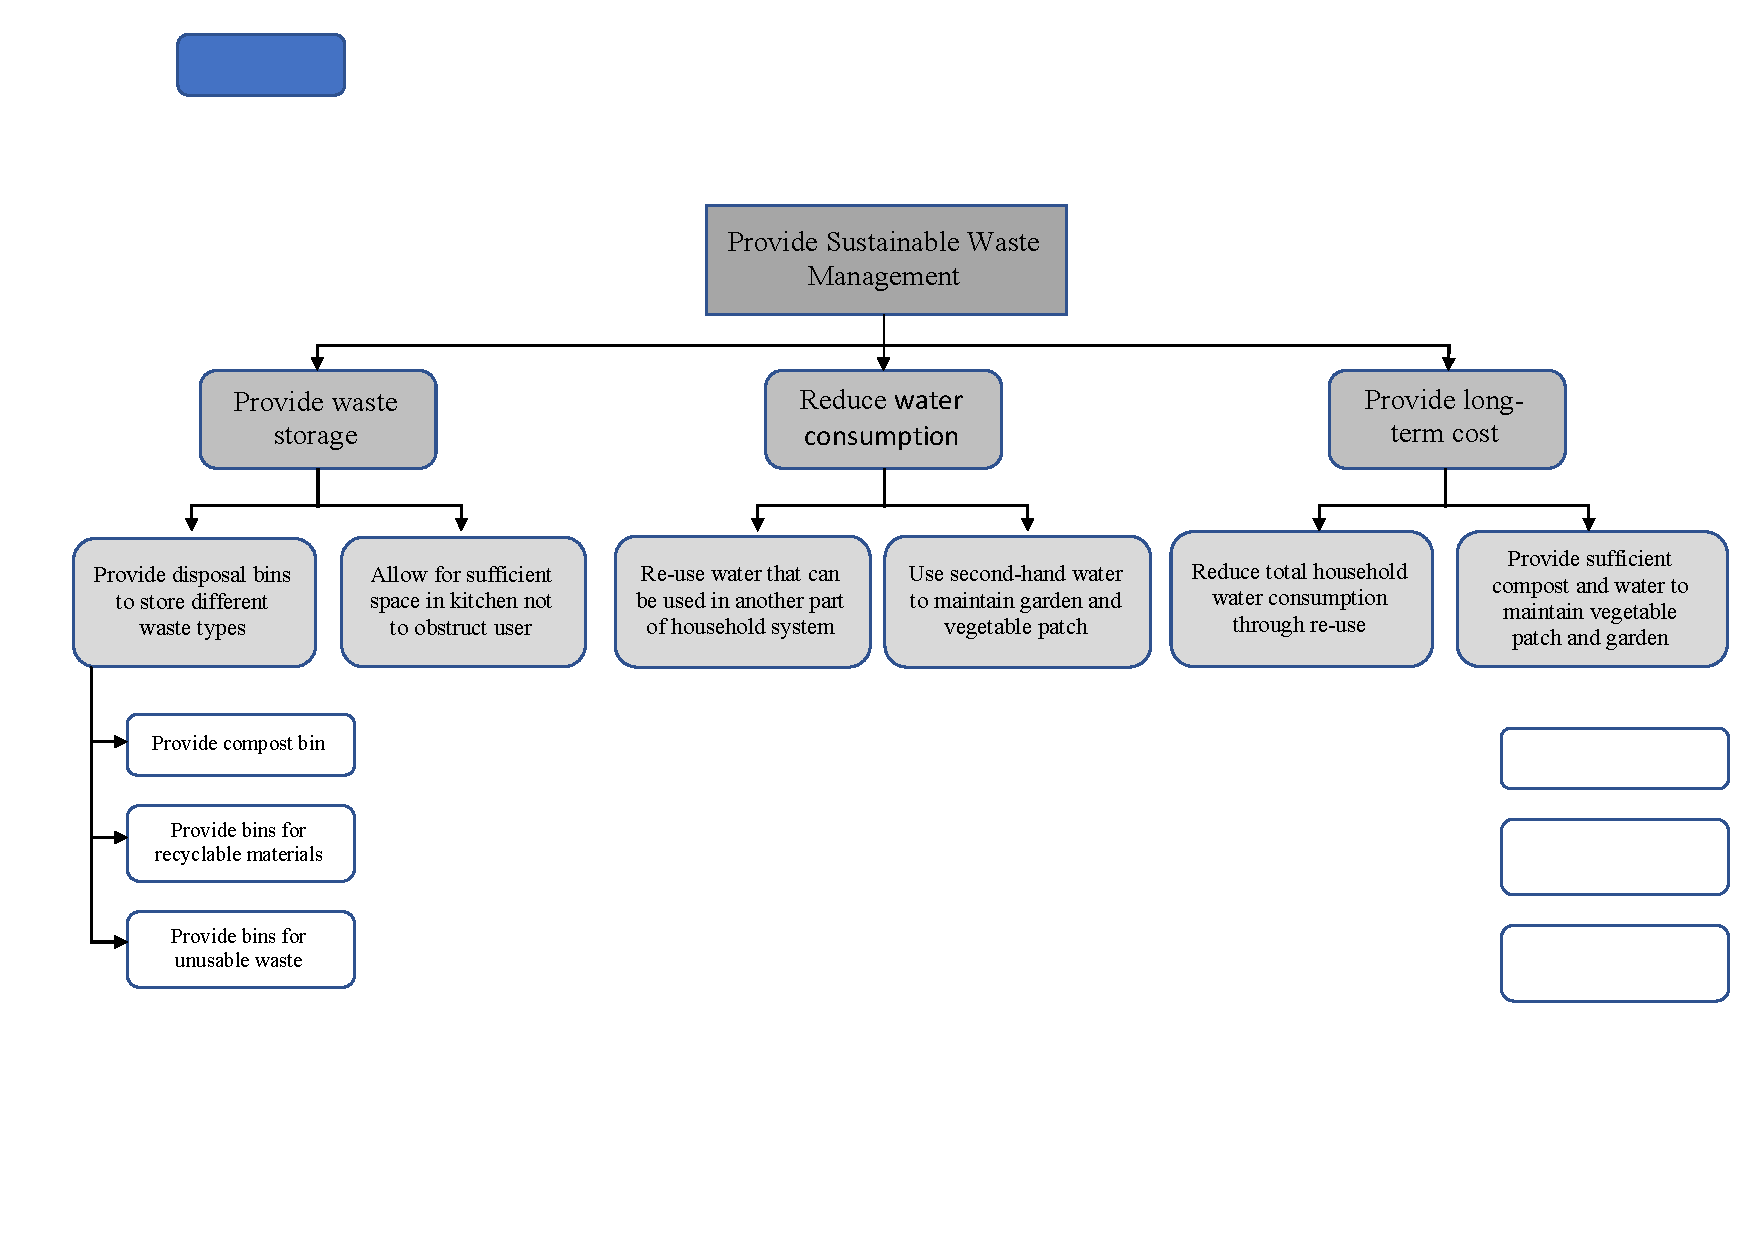
\includegraphics[scale = 0.55]{Objective_Tree_ecasa.pdf}
\caption{e-casa Objective Tree Structure}
\label{fig: ecasaOT}
\end{center}
\end{figure}

\subsection{Functional Definition}
\ac{e-casa} needs to perform the following functions in order to achieve the objectives layed out in the objective tree:\\

\noindent\textbf{Provide Waste Sortation and Storage} - The system must provide the capability for waste to be sorted according to its composition: paper, plastic, glass, organic material and unusable waste. Organic material must be reatained to be used in a composter and recyclable waste stored temporarily in its respective category for it to be later removed from the household system and passed on to the local municipality waste collection service.\\

\noindent\textbf{Reduce Water Consumption} - To achieve this objective a grey water system will need to perform the functions of receiving used water, processing this water (to be re-used again), storing the water until it is demanded at an outlet and directing the water from storage to the necessary outlet when it is demanded.\\

\noindent\textbf{Provide Long-term Cost Savings} - The use of a grey water system alone will provide long-term cost savings by means of reduced water consumption. Therefore if the objective of reduced water consumption is met with a grey water system that fulfills the necessary functionality, the household will demand less water from the municipality and cost savings will be realised immediately during system use. However, to provide long-term cost savings in other terms, \ac{e-casa} will need to effectively integrate grey water, composting and waste recycling to use each other's outputs as inputs and reduce the amount of external resources such as compost, vegetables and water to required to be used as inputs to the household system.

Effective utilisation (re-use) of water and organic waste will reduce the amount of water that needs to be purchased from the municipality, compost that needs to be purchased and eventually groceries that need to be bought. This functionality is essential to reduce the household's input costs and provide tangible finanacial value to the system user.

\subsection{Feasibility Definition}
At present there are household recycling bins available on the market that separate waste into the necessary categories. The technology is therefore currently available and feasible as a solution to the functions of waste sortation and storage. A recycling bin similar to that shown in Figure~\ref{fig: Household separation recycling bin} would likely be purchased and used in the \ac{e-casa} system.

\begin{figure}[h!]
\begin{center}
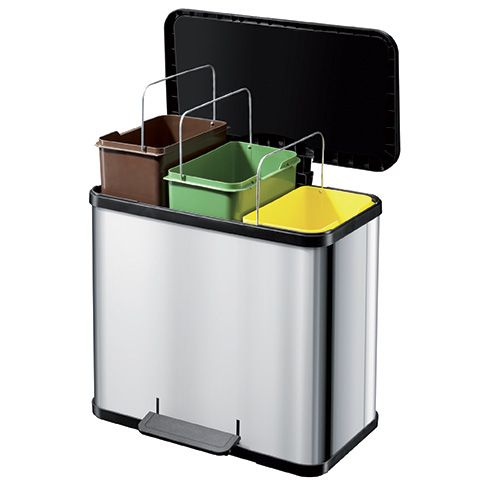
\includegraphics[scale = 0.34]{HouseholdRecyclingBin.jpg}
\caption{Household separation recycling bin}
\label{fig: Household separation recycling bin}
\end{center}
\end{figure}

There are also existing grey water systems available for purchase online or in-store. However, the setup of these systems and the size of its components usually vary case-to-case dependent on the appliances to be linked to the system, the size of the storage tank required by the household and the quality of the filtration component to be installed. Components of a grey water system can be easily purchased by any individual, but some degree of expertise and knowledge in the field is usually required to correctly size components, determine how they will function together and physically setup the system with the household's present water supply system. 

The design for \ac{e-casa}'s expected to be much like the one in Figure~\ref{fig: Grey water system} with linking to the household's shower/bath, basins, washing machine, outdoor tap and toilet.
%
\begin{figure}[h!]
\begin{center}
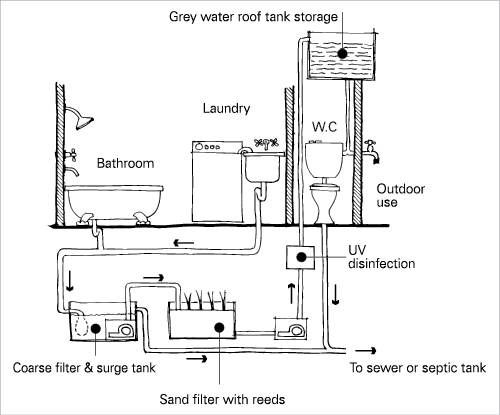
\includegraphics[scale = 1.15]{Household_Grey_Water.png}
\caption{Household grey water system}
\label{fig: Grey water system}
\end{center}
\end{figure}
%
A number of different household composters are available on the South African market. These composters are easily accessible and available online and in hardware stores. It is assumed for the time being that a 220 \textit{litre} composter (shown in Figure~\ref{fig: Outdoor Composter}) will be of sufficient size to store a household's organic and garden refuse waste.
%
\begin{figure}[h!]
\begin{center}
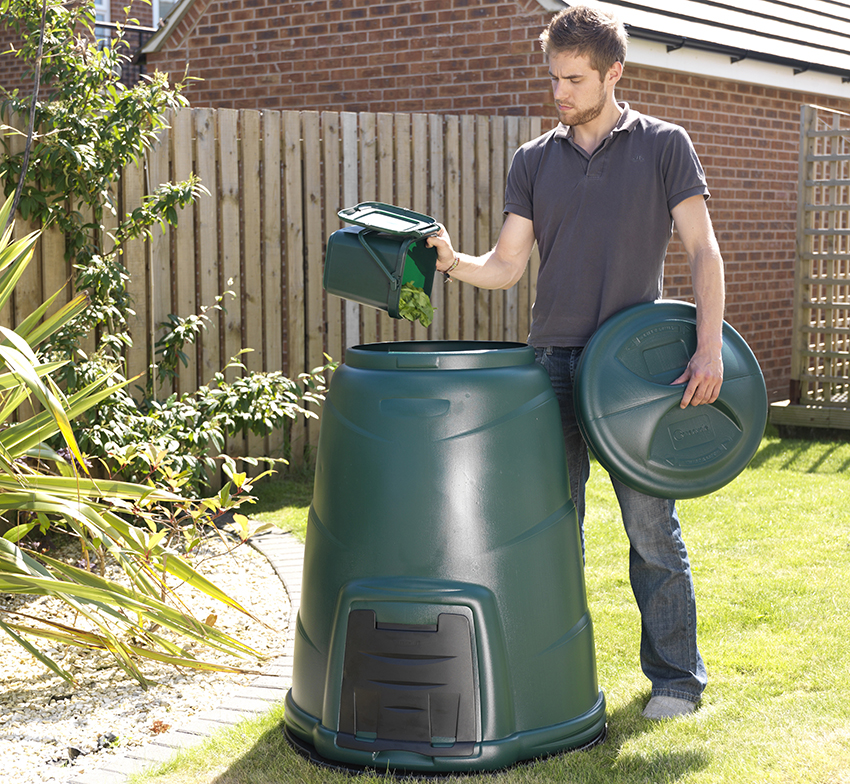
\includegraphics[scale = 1.1]{Outdoor_Composter.jpg}
\caption{Outdoor Household Composter (220 \textit{litres})}
\label{fig: Outdoor Composter}
\end{center}
\end{figure}

\subsection{Need Validation}
\textbf{Design Validation}
\textcolor{red}{What we need to do: Define metrics to evaluate performance rquirements. Present scenarios and evaluate what the metrics would do.}\\

To ensure the proposed system can fufill the identified need, metrics have been developed that will be used to evaluate the performance of the system.
%
\begin{table}[h!]
\caption {System Performance Metrics} \label{tb: Performance_Metrics} 
\begin{center}
\begin{tabular}{p{5cm}|p{3cm}|p{8cm}}\toprule
	{\textbf{Metric Category}} & {\textbf{Unit Measure}} & {\textbf{Description}}\\ \midrule
    Water savings & \textit{litres} & The volume of water saved is calculated as the reduction in the volume of water that enters the household. \\
    \hline
    Organic waste reduction & \textit{kilogram} & The total mass of organic waste re-used by means of composting is the reduction in household waste output.\\
    \hline
    Disposable waste reduction & \textit{kilogram} & The total mass of plastic, paper and glass respectively represent disposal waste reduction. It is assumed firstly, that all disposable materials were not previously recycled and that secondly, all disposable materials will be recycled by the municipality's garbage management system once the system is installed.\\
    \hline
    Household service cost saving & \textit{Rands} & The reduced water consumption of the household (from the municipality's system) and the re-used organic waste helps to perform household activities that would otherwise require a homeowner to purchase water, compost and vegetables. This includes the municipal water used in the household and compost for a vegetable garden. Household service cost saving is thus the total monetary savings obtained from reduced water use, self-composting and not having to purchase vegetables as frequently.\\
    \hline
    Payback Period & \textit{years} & The payback period is defined as the period of time it takes for the financial savings generated by the system, to equal the initial cost of purchasing and installing the \ac{e-casa} system. \\ \bottomrule
\end{tabular}
\end{center}
\end{table}
%
The five metrics in Table~\ref{tb: Performance_Metrics} are to be evaluated using different hypothetical scenarios. These scenarios reflect expected environmental conditions and consideration of the metrics in conjunction with these scenarios is used to determine the appropriateness of the system. The hypothetical scanarios are as follows:

\begin{description}
	\item[Long term system failure] - The water and waste savings will be realised within the first usage cycle, meaning once the system has re-used waste and waste, the saving immediately materialises. The return on investment is expected to be achieved before the onset of long term system failure. The likelihood of system failure can be decreased with continued maintenance of the system.
	\item[External market competition] - No other competitors are presently offering an integrated system however, there are suppliers offering parts of the system. This implies that other suppliers can match or better the household service cost of the \ac{e-casa} system. The reduced cost of implementing e-casa shall lie in the simple integration with current household systems. Customers would not require large renovations to install the system, reducing the over cost and improving the return on investment making the system marketable.
\end{description}

%As defined by the metrics, the system is believed to achieve the objectives laid out by the defined need. Thus the system is able to fufill the identified needs.

\section{Concept Exploration}
\subsection{Operational Requirements Analysis}
\textcolor{red}{analysing the stated operational requirements in terms of their
objectives. Restating, redefining or amplifying (as required) to provide specificity, independence and consistency among different objectives}

\subsection{Performance Requirements Formulation}
\textcolor{red}{Translating operational requirements into subsystem functions and defining a necessary and sufficient set of performance characteristics reflecting the functions essential to meeting the system’s operational requirements. Formulating the performance parameters required to meet the stated operational requirements.}

Subsystem functions are allocated and represented by the following \ac{FBD}s:\\
%
\begin{figure}[h!]
\begin{center}
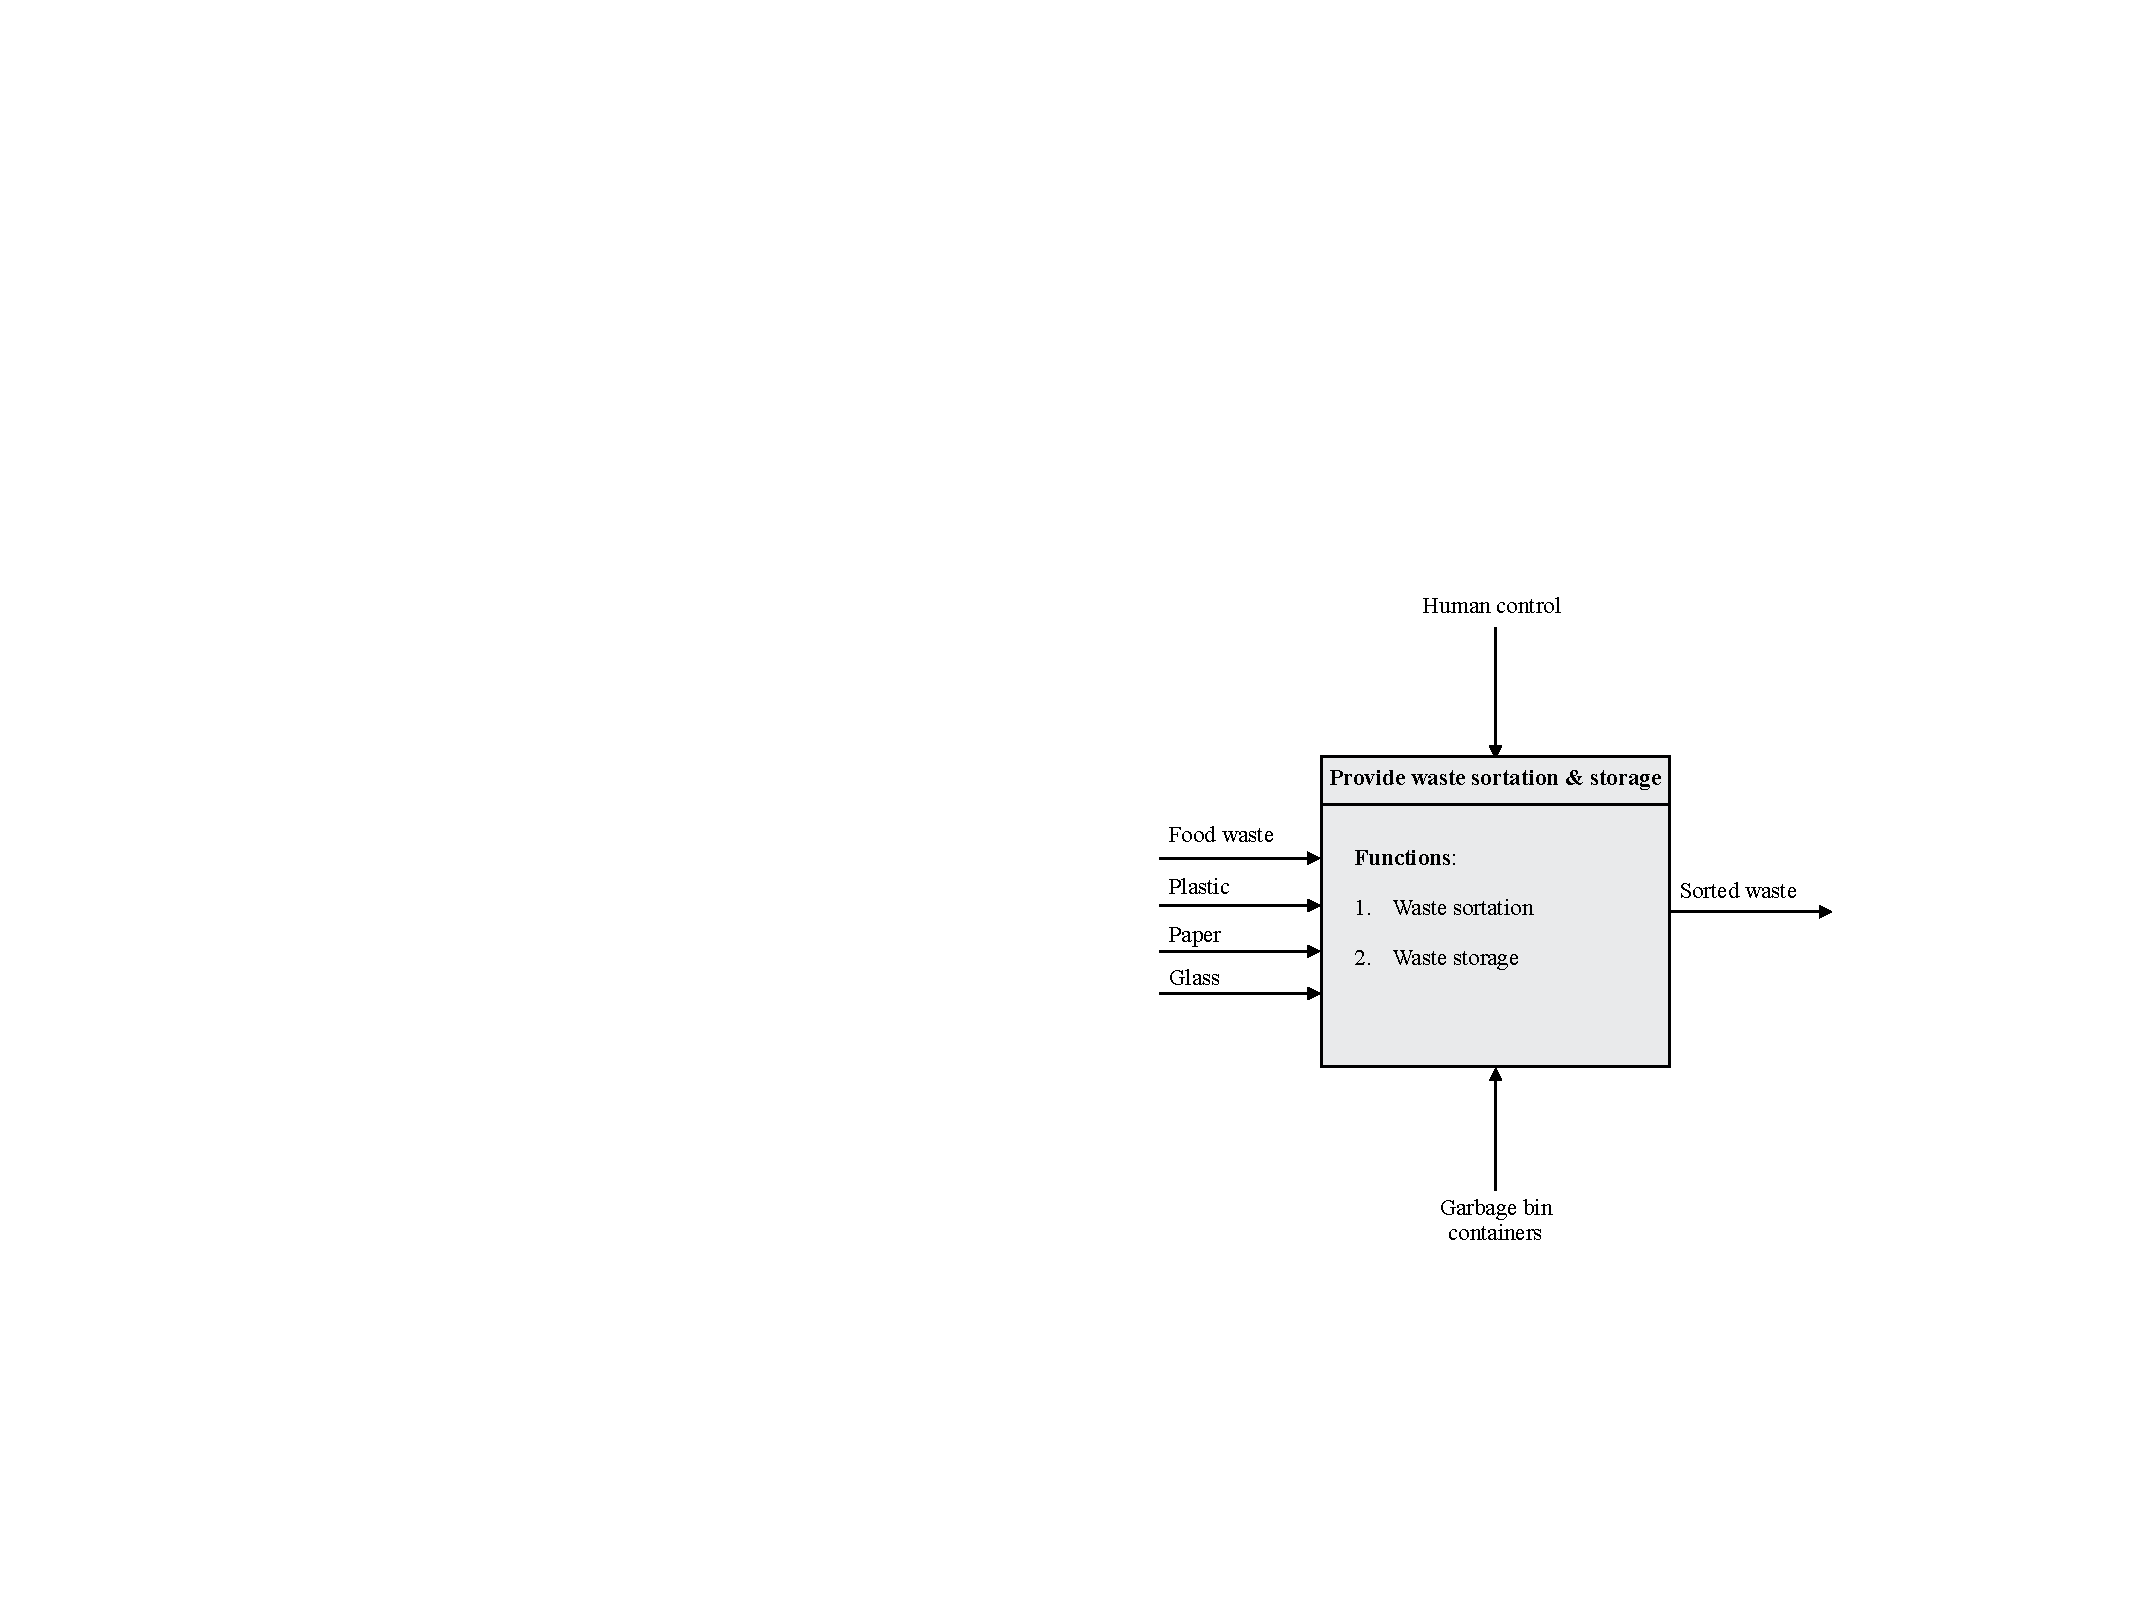
\includegraphics[scale = 0.7]{Function1.pdf}
\caption{Provide waste sortation and storage}
\label{fig: Function1}
\end{center}
\end{figure}
%
\begin{figure}[h!]
\begin{center}
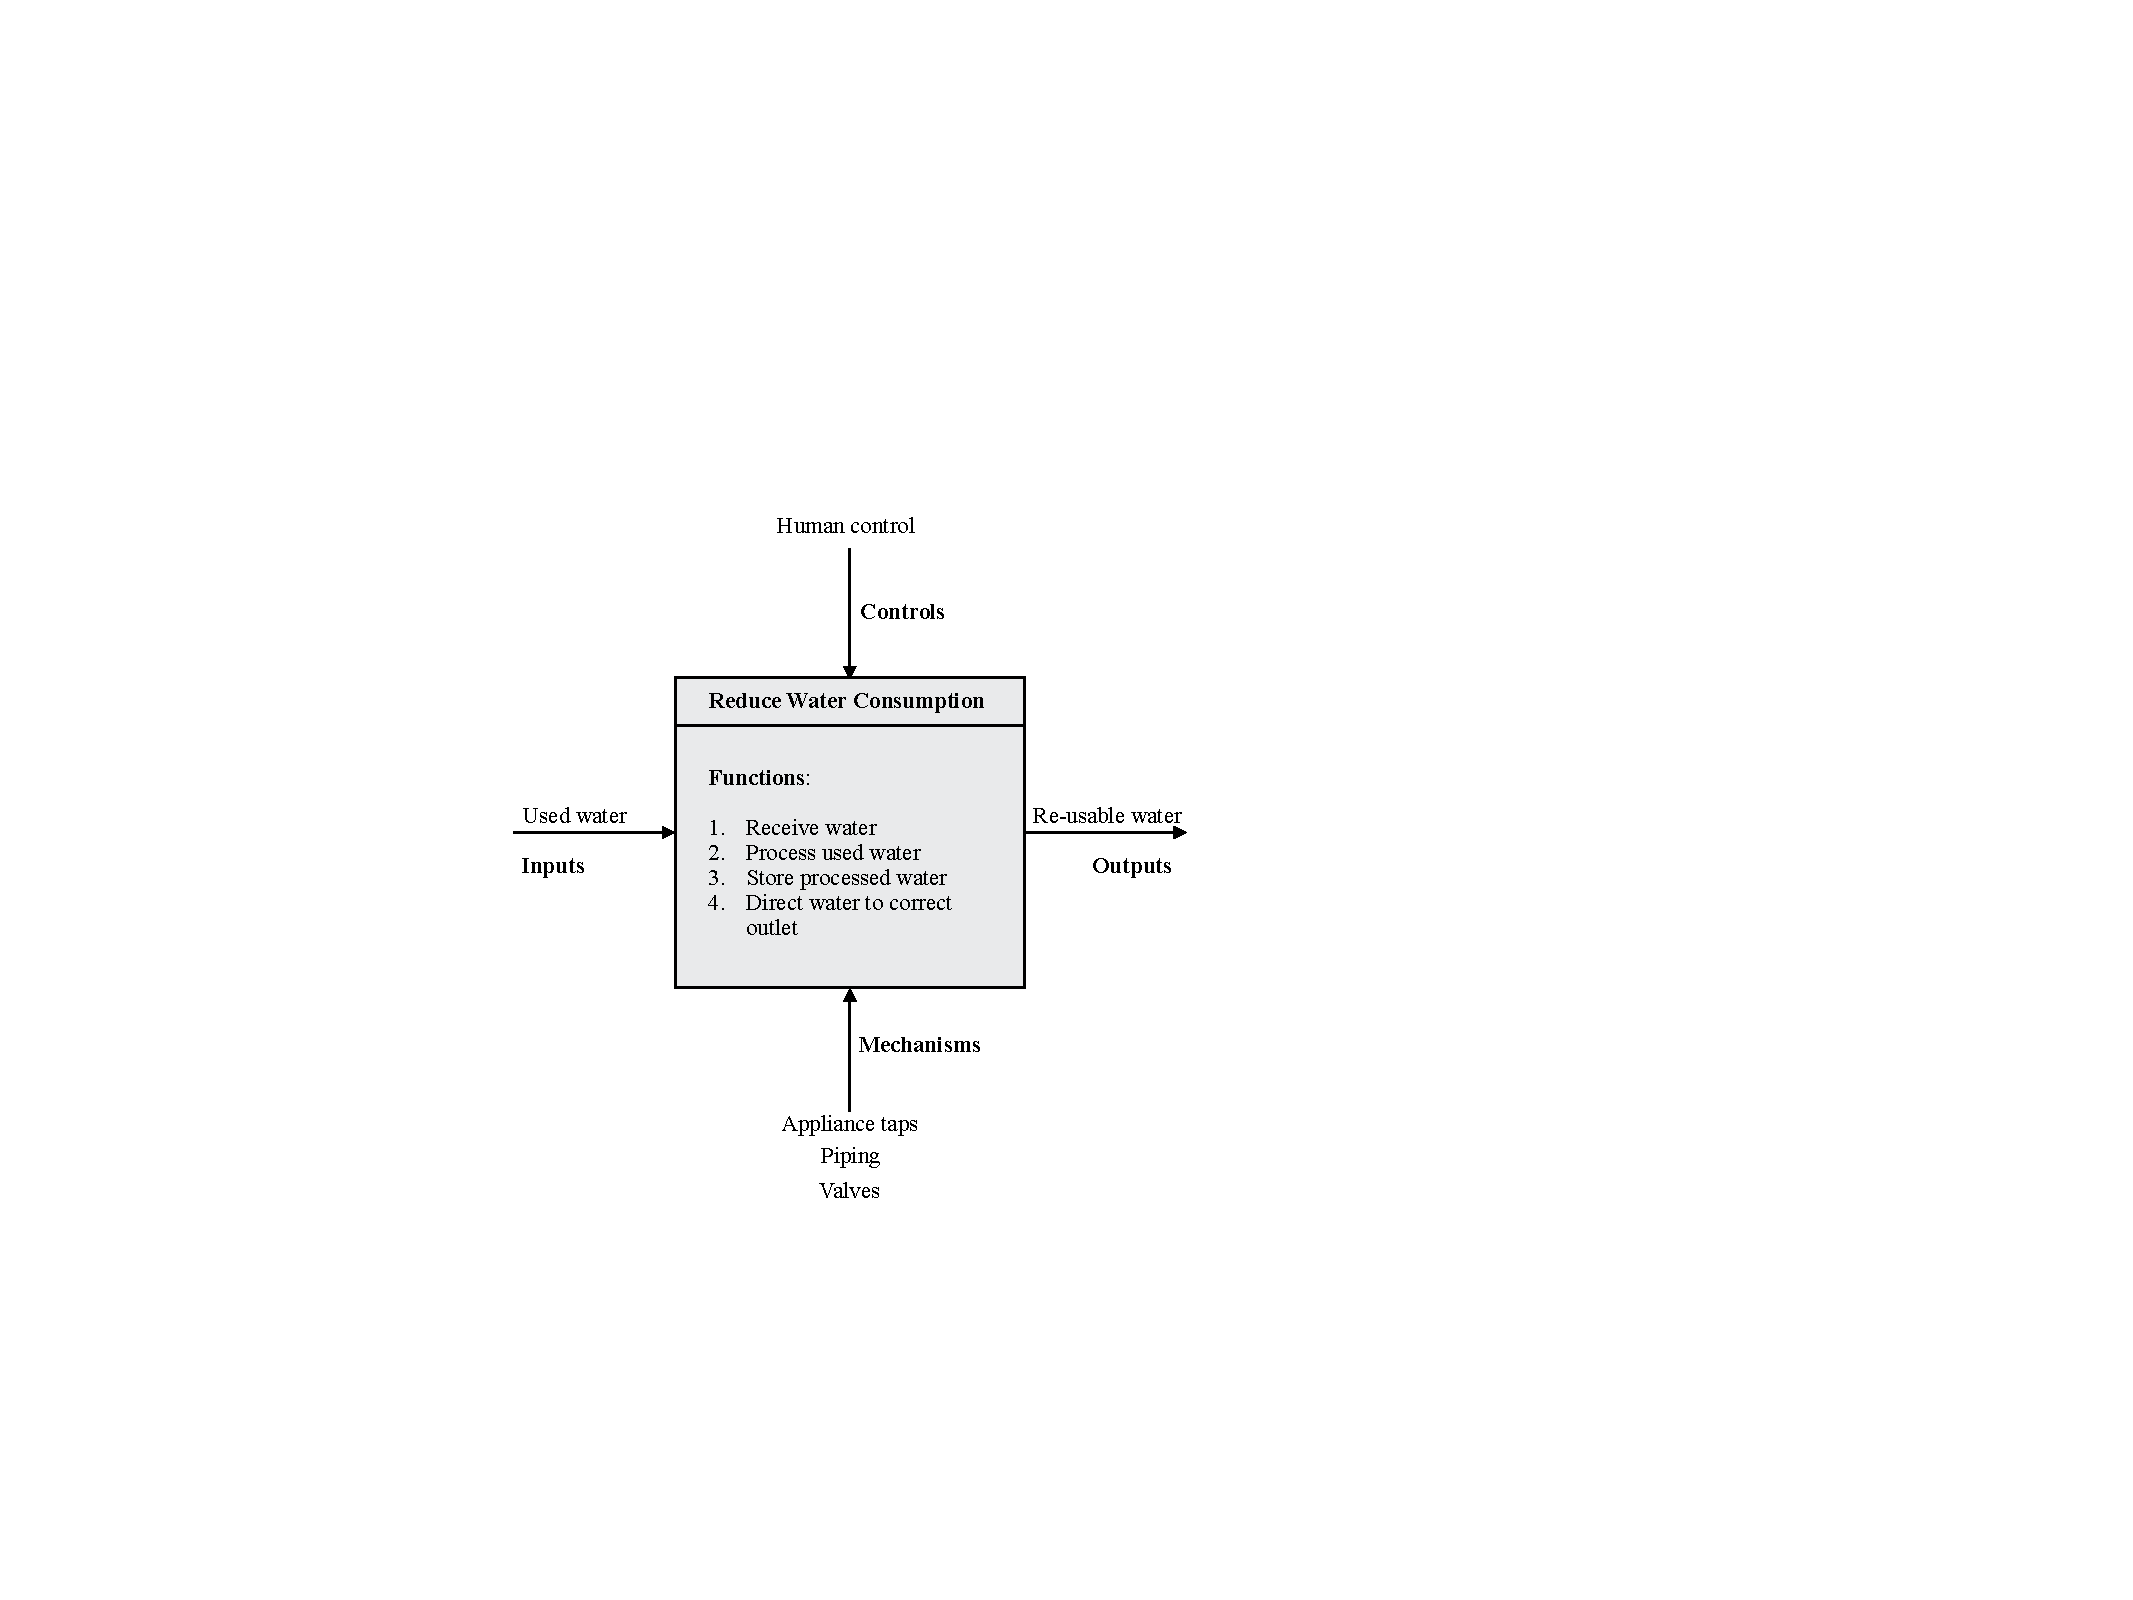
\includegraphics[scale = 0.7]{Function2.pdf}
\caption{Reduce water consumption}
\label{fig: Function2}
\end{center}
\end{figure}
%
\begin{figure}[h!]
\begin{center}
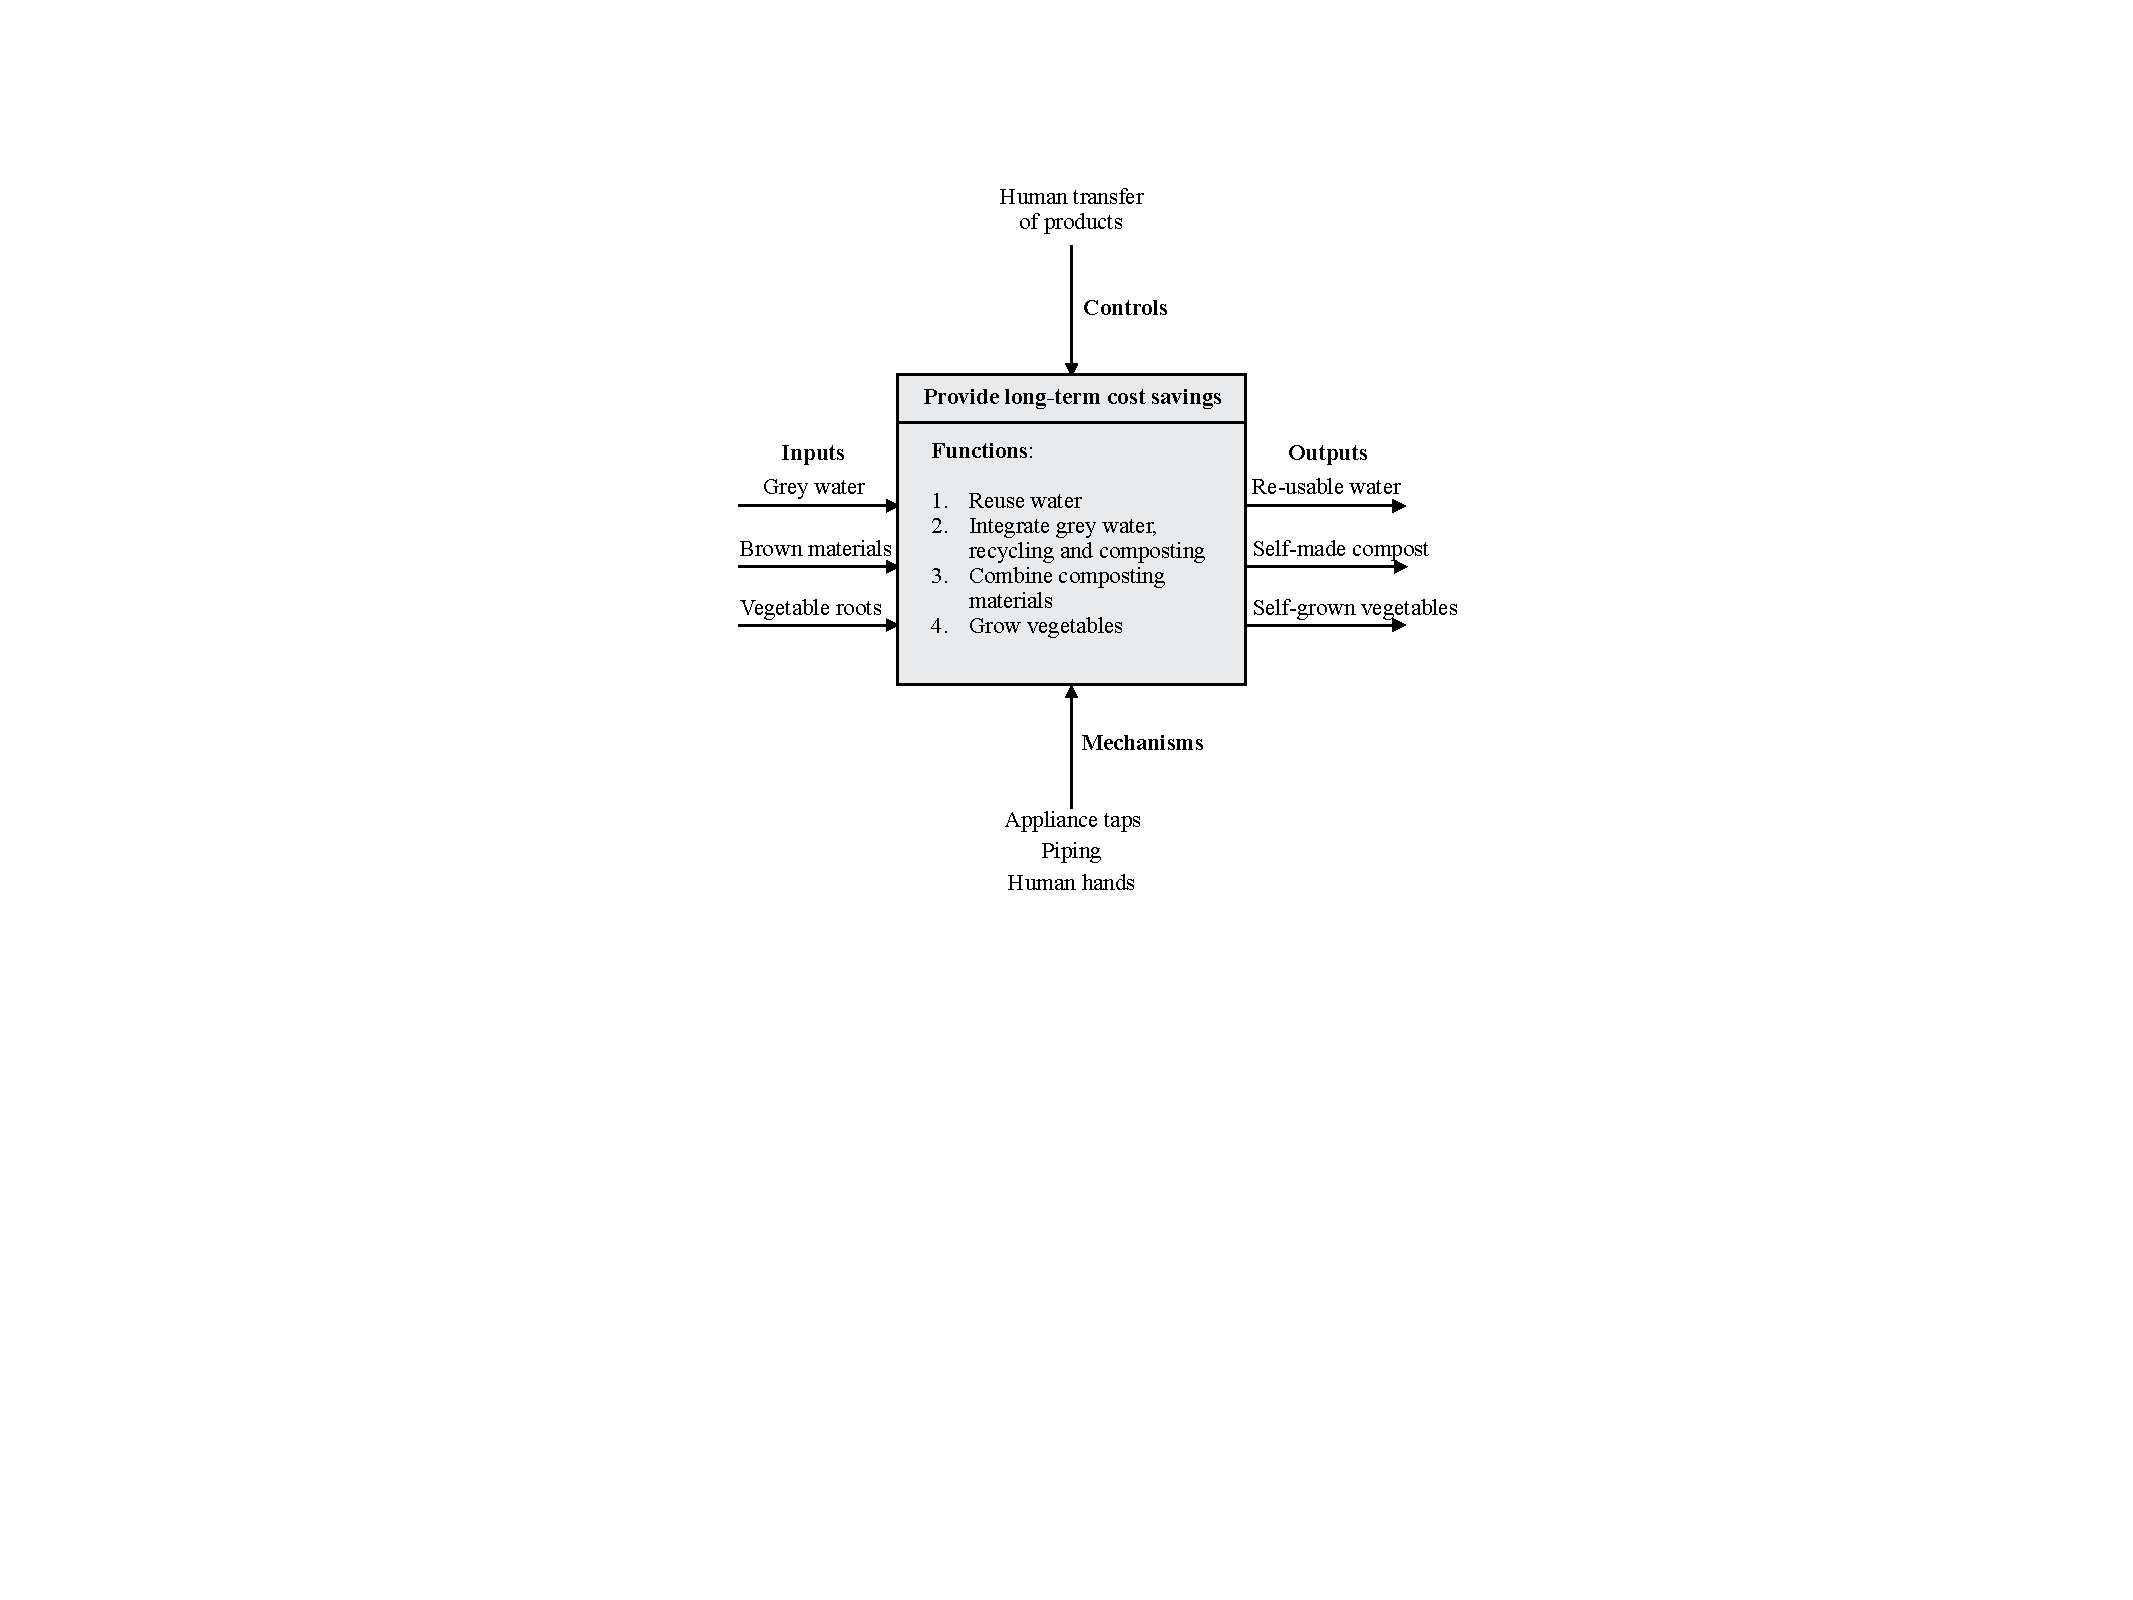
\includegraphics[scale = 0.7]{Function3.pdf}
\caption{Provide long-term cost savings function}
\label{fig: Function3}
\end{center}
\end{figure}

\subsection{Implementation of Concept Exploration}
\textcolor{red}{Exploring a range of feasible implementation technologies and concepts offering a variety of potentially advantageous options.}

%
\begin{table}[h!]
\caption {System Alternatives for Functional Tasks} \label{tb: Performance_Metrics} 
\begin{center}
\begin{tabular}{p{3.5cm}|p{6cm}|p{6cm}}\toprule
	{\textbf{Functional Task}} & {\textbf{Alternative 1}} & {\textbf{Alternative 2}}\\ \midrule
    Waste sortation & One garbage bin with multiple compartments & Multiple garbage bins each with a single compartment\\
    \hline
    Waste storage & a &The total mass of organic waste re-used by means of composting is the reduction in household waste output.\\
    \hline
    Receive water & Four separate pipes from (bath, shower, basin and washing machine) that connect to the central grey water storage tank & One pipe that merges bathroom appliance outputs and one kitchen pipe. These two pipes connect to the central grey water tank\\
    \hline
    Process used water & Filter grey water to be sent back to the washing machine for use & Do not purchase a filter and only use grey water in the garden for composting and plant watering\\
    \hline
    Store processed water & Large central tank to store all water received until it is needed again by the washing machine or in the garden & Small central tank to store used water only for the garden\\
    \hline
    Direct water & Three-way valve to direct grey water back to the washing machine, to the compost heap or to the household vegetable patch & \textcolor{red}{Don't know}\\
    \hline
    Re-use water & \textit{kilogram} & The total mass of plastic, paper and glass respectively represent disposal waste reduction. It is assumed firstly, that all disposable materials were not previously recycled and that secondly, all disposable materials will be recycled by the municipality's garbage management system once the system is installed.\\
    \hline
    Integrate water, recycling and composting & ... & ...\\
    \hline
     Combine composting materials & ... & ...\\
    \hline
     Grow vegetables & ...& ...\\
    \hline
    \bottomrule
\end{tabular}
\end{center}
\end{table}
%

\textbf{Recycling and Waste Disposal Technologies} - The recycling and waste disposal subsystem can be expanded to include metal and electronic waste bins as well. However, garbage bins with more than three bins to separate waste are not commercialy available and this type of garbage bin would therefore have to be designed and built. It is particulalry advantageous to simply purchase any already existent multiple-container garbage bin because the costs that would need to be incurred to design a new one do not appear to outweigh the financial or intangible benefits to be gained. It is also expected that most households will not have enough physical space to house such a large bin and if a household did, it would be easy to purchase two three-container bins for use. Furthermore, metal and electronice waste is often found in significantly smaller quantities than more populous, plastic, paper and glass waste and it is difficulty to justify separate containers for these two waste categories as they will likely only be emptied a couple times a year.\\

\textbf{Grey water system technologies} - 
	
	
\textbf{Composting Options} - 
	

\subsection{Performance Requirements Validation}
\textcolor{red}{Conducting effectiveness analyses to define a set of performance requirements that accommodate the full range of desirable system concepts and validating the conformity of these requirements with the stated operational objectives and refining the requirements if necessary.}

The most suitable alternative for each of the system aspects addressed in the section above will be chosen to form the the system. The system as whole must be as cost effective as possible. However, quality should not be sacrificed for unreliable components. The grey water system components will be selected with the intention of a minimum 50 year project life for each, as per industry piping standards. %\cite{Fischer2012}. this ref is giving erros
This is important to ensure the system does require repairs over the life of the project, only maintenance. The labour and expertise required to make system repairs for the installed grey water system are expected to be costly and should be avoided.

as it will need to be used by people who may be technologically challenged. The most attractive alternative that has been selected as feasible and appropriate is described below.
The alternatives chosen to fulfil the functioning tasks are the biometric scanner for fingerprinting, a touch screen for the data input, a receipt printer and portable card machine for payments as well as a cash alternative feed, a built-in camera and scanner to take pictures and to scan documents and lastly, a hard drive for the data storage. These alternatives were chosen with the multi objectivity of suitability, convenience, ease of use and a consideration of cost effectiveness in terms of meeting the requirements without over-designing for its purpose.

%====== Current Session
\section{Concept Definition}
\subsection{Performance Requirement Analysis}
\subsubsection{Relating analysed spesifications to operation needs}
Three primary operational needs were identified. Each need will be evaluated individually to determine if the proposed spesifications can adhere to the need.

\begin{enumerate}
    \item Reduce water consumption
    \begin{enumerate}
        \item Reducing the amount of water consumed by a household would require that water be reused when possible. The specification states that \textcolor{red}{10\%} of input water be diverted to other functions within the house thus reducing the water used from the municipal supply. The net effect is that less water is purchased from the municipality and the consumption decreases.
    \end{enumerate}
    \item Reduce the production of physical waste
    \begin{enumerate}
        \item The production of physical waste refers the mass of waste that a house outputs and the municipality receives to be processed. Composting organic waste reduces the mass of waste the municipality must process and thus reduces the net waste produced by a house hold.
        \item Sortation of waste into paper, plastic or glass permits recycling companies to use the various materials and thus reduces the amount of waste required to be processed by the municipality. 
        \item The net redution of waste is required to be \textcolor{red}{20\%}
    \end{enumerate}
    \item Provide sustainable waste management system
    \begin{enumerate}
        \item Reducing the amount of water consumed by a household directly reduces the running cost of the house and thus for cost reduction to occur, further reductions in water consumption are required. The reduction in costs of the waste management system shall only materialse once the the composting has been compete. Households may used the composite for the maintenance of their gardens or to grow their own vegatbles, further reducing household running costs. A cost reduction of \textcolor{red}{13\%} is anticipated as the impact of reducing physical waste priduction has less direct implications on cost.
        \item the cost of the system is expected to fairly high. The savings, in the form of reduced operating costs of a household, generated by the system must be repaid within a \textcolor{red}{2 year period}.
        \item Reducing the comsumption of water and production of physical waste reduces the net effect on the environment. This achived goal of \textcolor{red}{5 ton reduction}.
    \end{enumerate}
\end{enumerate}

Water usage reduction - the water usage can e reduced by the amount spesified.
Waste usage reduction - the waste can be reduced by the amount spesfied
Cost saving - cost sagin can be achived if the first two spesifications are achvied
Net return of investment - the efficiency of the cost saving will determine if the system can pay itself off within 3 years. 




\subsection{Functional Analysis and Formulation} 
\textcolor{red}{Allocating subsystem functions to the component level in terms of system functional elements and defining element interactions, developing functional architectural products, and formulating preliminary functional requirements corresponding to the assigned functions.}

\subsection{Concept Selection}
\textcolor{red}{Synthesizing alternative technological approaches and component configurations designed to performance requirements; developing physical architectural products; and conducting trade-off studies among performance, risk, cost, and schedule to select the preferred system concept, defined in terms of components and architectures.}

\subsection{Concept Validation}
\textcolor{red}{Conducting system analyses and simulations to confirm that the selected concept meets requirements and is superior to its competitors and refining the concept as may be necessary.}

\chapter{Engineering Development Phase}
\textcolor{red}{analysing the system functional specifications with regard to their derivation from operational and performance requirements and the validity of their translation into subsystem functional requirement identifying components requiring development}

The system's functional specifications are translated into three subsystem functional requirements:\\

\textbf{Grey Water subsystem} - This system interfaces with the household's municipal water supply which is its primary input. It is also connected to multiple household components, namely: the washing machine, bath/shower, toilet cistern and garden. This subsystem has three functional capabilities. The first being to store grey water in a central tank to be recycled (re-used) in the system, secondly to sort re-usable water from unusable waste water and finally to transfer both the re-usable and unusable water in the subsystem to the appropriate destination (component). This subsystem also feeds grey water to the next subsystem (compost).\\

\textbf{Compost subsystem} -  The compost subsystem interfaces with the household's garden and organic material stockpile components. It uses organic materials from the material stockpile to provide compost to the garden component. It's primary capabilities are to store organic materials and provide some form of visual management for the user to know when there is sufficient compost for the storage container to be emptied. This subsystem is connected to the grey-water subsystem which provides grey water as an input as well as to the Recycling and waste disposal subsystem which provides paper and other organic waste to the compost system.\\

\textbf{Recycling and waste disposal subsystem} - This subsystem interfaces with the household's kitchen as a component in order to receive all household waste as an input. It also intrefaces with the municipal recycling system at the point where waste is placed on the sidewalk for collection by the municipality's waste collection service. Its primary capability is to sort household waste into the relevant categories for re-use or disposal. Paper recyclables and organic waste collected by this subsystem are output to be used in the compost subsystem while other recyclables and non-recylable waste is disposed of to the municipal recycling system.


\begin{figure}[h!]
\begin{center}
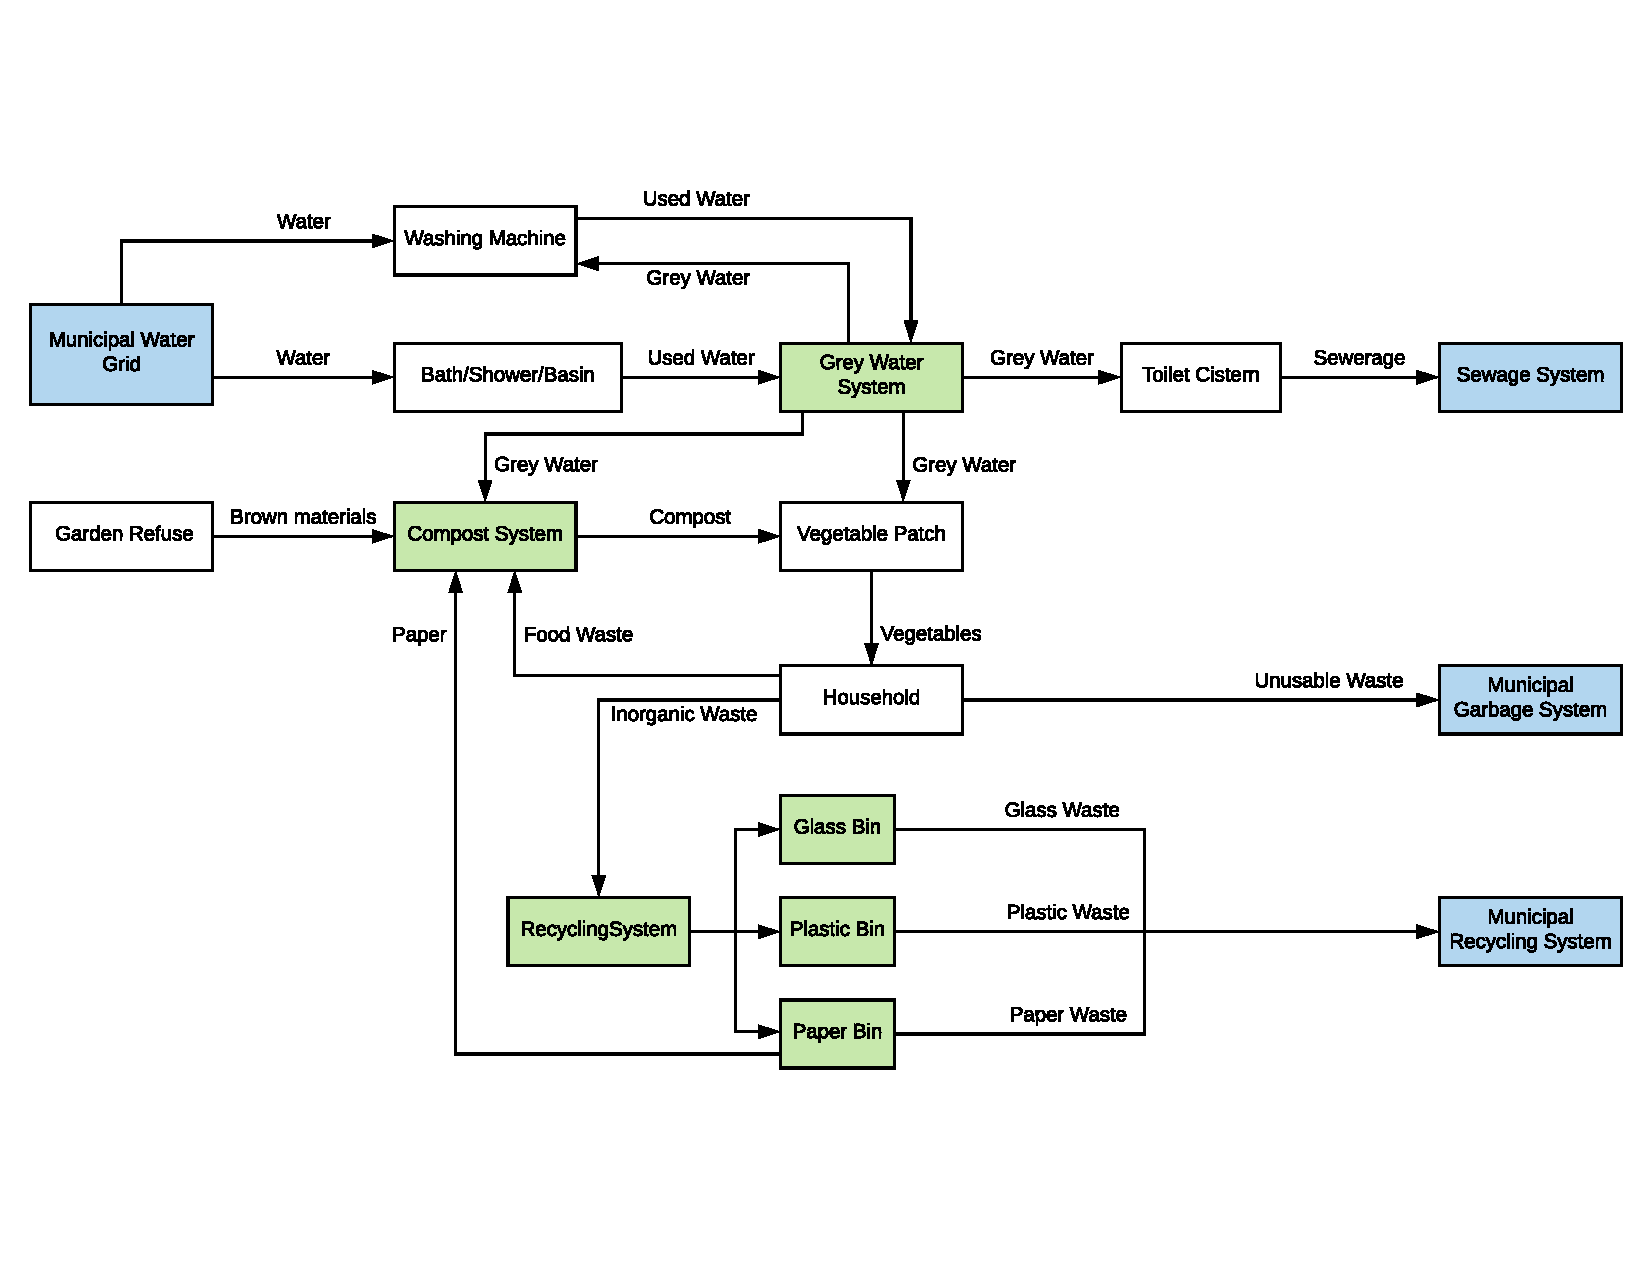
\includegraphics[scale = 0.55]{System_Diagram.pdf}
\caption{System Diagram}
\label{fig: systemDiagram}
\end{center}
\end{figure}


\section{Advanced Development Phase}

\subsection{Requirements Analysis}

\subsection{Functional Analysis and Design}

\subsection{Prototype Development}

\subsection{Development Testing}

\section{Engineering Procurement Phase}

\subsection{Requirements Analysis}

\subsection{Functional Analysis and Design}

\subsection{Component Design}

\subsection{Design Validation}

\section{Integration and Evaluation Phase}

\subsection{Test Planning and Preparation}

\subsection{System Integration}

\subsection{Developmental System Testing}

\subsection{Operational Test and Evaluation}

\chapter{Post Development Stage}

\section{Production and Deployment Phase}

\subsection{Transitions from Development to Production}

\subsection{Production Operations}

\section{Operations and Support Phase}
\textcolor{red}{Installation and test (system integration site, internal and external, disruptive or non-disruptive installation, early system operational difficulties encountered or that could be encountered, operational personnel)
Logistics, Support and Maintenance schedule
System Upgrades (hard and software upgrade plans)}

\chapter{Software Design and System Dynamics}
\textcolor{red}{This phase is required to study the behaviour and structure of a system by carrying out sensitivity analysis tests. Only select critical elements or more as deemed fit from the designed system and apply to these to the modelling capability of a chosen software.
Your algorithm/software approach should be such that a change in the value of one element’s input can be quantitatively seen in other elements within the network. [Use software such as: Anylogic, Vensim, Stella, Dynamo++ etc]
Phase II is tied to your ability to demonstrate sensitivity analysis, structure and behaviour of a system resulting from a change in one or more parameters of some system elements.}

\section{Core 9 System Design Structure}

\section{System Dynamics Analysis}
==35marks==

\section{Selected Elements for System Dynamics Analysis}
==10/35marks==
Reason for selecting these elements in a situation where the new network for SD differs from the main designed network ==5/35marks==

\section{Sensitivity Analysis}
==20/35marks==
Simulation runs to demonstrate sensitivity analysis, changed system behaviour etc 

\chapter{Conclusion}
\acresetall
  

\bibliography{References}

\appendix
\chapter{Some data as appendix}

\end{document}

%A water re-use function must be provided to discern which water must be retained by the hosehold for use and which must be discarded into the municipal system based on the origin of the water. ie. Waste water from the toilet must be discarded into the municipal system but used water from the bathroom sink must be retained for re-use to flush the toilet or water the household vegetable patch. This function will also add value to the local municipality by reduce waste output and the volume of water that must be processed.\\

%\begin{description}
%	\item[Water savings (\textit{litres})] - The volume of water saved is calculated as the reduction in the volume of water that enters the household. 
%by the volume of water diverted into the grey-water system and represents a direct saving to the user.
%	\item[Organic waste reduction (\textit{kg})] - The total mass of organic waste re-used by means of composting is the reduction is household waste output.
%	\item[Disposable waste reduction (\textit{kg})] - The total mass of plastic, paper and glass respectively represent disposal waste reduction. It is assumed firstly, that all disposable materials were not previously recycled and that secondly, all disposable materials will be recycled by the municipality's garbage management system once the system is installed.
%	\item[Household service cost saving (\textit{Rands})] - The reduced water consumption of the household (from the municipality's system) and the re-used organic waste helps to perform household activities that would otherwise require a homeowner to purchase water, compost and vegetables. This includes the municipal water used in the household and compost for a vegetable garden. Household service cost saving is thus the total monetary savings obtained from reduced water use, self-composting and not having to purchase vegetables as frequently.
%	\item[Payback Period (\textit{years})] - The payback period is defined as the period of time it takes for the financial savings generated by the system, to equal the initial cost of purchasing and installing the \ac{e-casa} system. 
%\end{description}
